
\documentclass[12pt]{article}

%пакеты для работы с кириллицей
\usepackage[english,russian]{babel}
\usepackage{cmap}
\usepackage[utf8]{inputenc}
%\usepackage{fixltx2e}
\usepackage{mathtext}
\usepackage{rotating}
\usepackage[a4paper,top=1cm,bottom=2cm,left=3cm,right=3cm,marginparwidth=1.75cm]{geometry}
%%% Работа с русским языком
\usepackage{cmap}          % поиск в PDF
\usepackage{mathtext}         % русские буквы в фомулах
\usepackage[T2A]{fontenc}      % кодировка
\usepackage[utf8]{inputenc}      % кодировка исходного текста
\usepackage[english,russian]{babel}  % локализация и переносы
\usepackage{pgfplots}
\usepackage{comment}

\usepackage{graphicx}      % tools for importing graphics
%\usepackage{lgrind}        % convert program code listings to a form 
                            % includable in a LaTeX document
%\usepackage{xcolor}        % produces boxes or entire pages with 
                            % colored backgrounds
%\usepackage{longtable}     % helps with long table options
%\usepackage{epsf}          % old package handles encapsulated postscript issues
\usepackage{bm}            % special bold-math package. usge: \bm{mathsymbol}
%\usepackage{asymptote}     % For typesetting of mathematical illustrations
%\usepackage{thumbpdf}
\usepackage{caption}

\usepackage{titlesec}
\usepackage[dotinlabels]{titletoc}

\usepackage[siunitx]{circuitikz} %рисование схем
\usepackage{mathrsfs} %значок ЭДС
\usepackage{svg} %добавление .svg картинок
\usepackage{longtable} %таблица2
\usepackage{float} %насильное положение таблиц
\usepackage{titling} %аннотация после названия
\usepackage{wrapfig} %возможность ставить картинки рядом с текстом
\usepackage{indentfirst} %отступ у первого предложения после начала параграфа
\usepackage{multirow} %extra для таблиц
\usepackage{rotating} %повернутые фигуры в конце документа
\usepackage{longtable} %разделяемые на несколько страниц таблицы
\usepackage{titlesec} %subsubsections
\usepackage{amsmath}
\usepackage{geometry}

\usepackage{subcaption}
\captionsetup{compatibility=false}

\usepackage{array}

\usepackage[hidelinks]{hyperref}  % this package should be added after 
                                        % all others.
                                        % usage: \url{http://web.mit.edu/8.13}

\setcounter{secnumdepth}{4}

\begin{document}
\begin{titlepage}


\begin{center}
 {\large Московский физико-технический институт (МФТИ-Физтех)}
\vspace{9cm}

{\Large Лабораторная работа 1.1.8:\\ Измерение ускорения свободного падения при помощи падения сферического магнита} \\[0.5cm] % название работы, затем отступ 0,5с
\ Иванов Артём, Б05-409\\[0.5cm]
%\email{nobody@mit.edu}
%\homepage{http://web.mit.edu/8.13/} %If you don't have one, just comment out this line.
\today
%\affiliation{Московский Физико-техничесикй Институт}
\end{center}
\end{titlepage}

\newpage

\section{Цель работы:}
Определить ускорение свободного падения посредством прямых измерений ускорения падающего тела.

\section{Оборудование:}
Вертикальная труба с намотанными катушками; шарообразные
неодимовые магниты; линейка; блок регистрации сигнала (микроконтроллер с АЦП), соединённый с цифровым осциллографом.

\section{Теоретические сведения}
В данной работе ускорение свободного падения $g$ определяется при помощи измерения времени падения металлического шарика в поле тяжести Земли.

Рассмотрим падение шарика из его начального положения, когда он удерживается электромагнитом. Направим ось у вертикально вниз, а начало отсчёта  $v_0 = 0$ совместим с положением самой верхней катушки.
Пусть $v_0$ – скорость шарика в центре самой верхней катушки. Для равноускоренного движения шарика справедливо выражение:
\begin{equation}\label{сигма}
y = v_0 t + \frac{gt^2}{2}
\end{equation}
Выражение (1) можно записать для пяти моментов времени $t_n$ (n = 1, 2, 3, 4, 5) ,соответствующих пролёту шарика через соответствующую катушку:
\begin{equation}\label{сигма}
nl = v_0 t_n + \frac{gt_n^2}{2}
\end{equation}
Перепишем выражение (2) в виде:
\begin{equation}\label{сигма}
\frac{nl}{t_n} = v_0 + \frac{gt_n}{2}
\end{equation}
\newpage
Проводя измерения времён $t_n$ при свободном падении шарика и используя выражение (3), можно построить график зависимости величины $nl/t_n$ от $t_n$ и определить ускорение свободного падения из углового коэффициента данной зависимости.\\

\begin{center}
    \textbf{Влияние сопротивления воздуха}
\end{center}

При падении с малыми скоростями можно применить известную формулу Стокса:
\begin{equation}
F_{сопр} = 6 \pi\mu r v
\end{equation}
где $r$ — радиус шара, $\mu$ — вязкость воздуха (при нормальном  давлении и комнатной температуре $\mu \approx$ 1,85 $\cdot 10^{-5}$ Па $\cdot$ с).
При больших скоростях обтекание шарика становится турбулентным и теория Стокса неприменима. Сила оказывается пропорциональна квадрату скорости и площади поперечного сечения шарика:
\begin{equation}\label{сигма}
F_{сопр} = C \cdot \pi r^2 \rho v^2
\end{equation}
где $\rho$ — плотность воздуха ( $\rho \approx 1,2 \text{кг}/\text{м}^3$ ), $C$ — константа, зависящая от формы тела, которая для может быть установлена только экспериментально.
Для шара известно экспериментальное значение $C_{ш}\approx 0,2$. Заметим, что формула (5) имеет прозрачный физический смысл: величина $C \cdot \pi r^2 \rho v^2$ — это количество импульса, которое сообщали бы в секунду молекулы воздуха шарику при
неупругом ударе о него (убедитесь в том самостоятельно).

Критерием выбора между двумя моделями служит так называемое число Рейнольдса
\begin{equation}\label{сигма}
Re = \frac{\rho v r}{\mu}
\end{equation}

\section{Результаты измерений и обработка данных}
Диаметр шара $d=(30.0 \pm 0.1)\text{мм}$

Масса шара $m=(107.3 \pm 0.1)\text{г}$

Расстояние между датчиками $l=(40.0 \pm 0.1)\text{см}$

В Таблице 1 приведенны результаты измерений с помощью датчика с АЦП.

В Таблице 2 приведенны результаты измерений с помощью курсоров на осциллографе.

На Рис.1 изображен поиск времен с помощью курсоров

Заметим, что значения полученные курсорами не сильно отличаются от значений с помощью АЦП, однако значения с помощью АЦП значения получаются с большей точностью. Поэтому будем использовать значения полученные с помощью АЦП.

Построим графики $nl/t_n(t_n)$ для каждого №, по угловым коэффициентам определим $g$ и усредним.

На Графиках представленны все зависимости.

Методом МНК для линейной регрессии определим угловые коэфициенты и свободные члены.

Уравнение регрессии: $\frac{nl}{t_n}(t_n) =  b + k\cdot t_n$.

Занесем полученые данные в Таблицу 4. Также в эту же таблицу занесем даные для максимальных значений чисел Рейнольдца для каждого опыта.

Если маскимальное число Рейнольдца $Re_{\max} < 1000$, то на протижении всего опыта обтекание воздухом ламинарное.
\[Re_{\max}=\frac{v_{\max}\rho r}{\mu}\]
где
\[v_{\max} \approx v=\frac{\Delta L}{\Delta t}=\frac{l}{t_5-t_4}\]

Из Таблицы 4 видно, что число $Re_ {\max}>1000$, это значит, что на части пути обтекание ламинарное, а на части турбулентное.

Рассчитаем силу сопротивления по формулам, для $v_{\max}$ и занесем данные в Таблицу 5.

По сравнению с $2k$ все $a_\text{л}$ и $a_\text{т}$ пренебрежимо малы ($<1\%$).

Усредним все полученные $k$, рассчитаем $g_\text{ср}$ и найдем среднеквадратичное отклонение как статистическую погрешность.

\[g=2k_\text{ср}=2\cdot505.5\text{см}/\text{с}^2=10.11\text{м}/\text{с}^2\]
\[\epsilon_g=\epsilon_k=\frac{\sigma_k}{k_\text{ср}}=\frac{8.3}{505.5}=1.6\%\]
\[\sigma_g=1.6\%\cdot g=0.16\text{м}/\text{с}^2\]
\underline{$g = 10.11 \pm 0.16 \frac{\text{м}}{\text{с}^2}$, $\varepsilon = 1.6\%$}
\section{Вывод}

Нам удалось успешно измерить ускорение свободного падения с хорошей точностью (погрешность порядка $1.6\%$), причем полученное значение с учетом погрешности попадает в табличное.
\newpage
\section{Графики и таблицы}
\begin{table}[h!]
\centering
\begin{tabular}{ |p{0.6cm}|p{1.2cm}|p{1.2cm}|p{1.2cm}|p{1.2cm}|p{1.2cm}| }
\hline
№ & $t_1, \text{мc}$ & $t_2, \text{мc}$ & $t_3, \text{мc}$ & $t_4, \text{мc}$ & $t_5, \text{мc}$ \\
\hline
1&	118.48&	207.21&	283.01&	349.94&	410,37\\
\hline
2&	118.81&	207.16&	282.86&	349.71&	410,13\\
\hline
3&	117.42&	207.09&	283.42&	350.72&	410,74\\
\hline
4&	117.22& 207.40& 285.36& 347.70& 408,66\\
\hline
5&	117.13& 206.98& 283.56& 351.56& 412,09\\
\hline
6&	117.00& 207.15& 285.07& 348.07& 409,29\\
\hline
7&	117.67& 207.09& 283.21& 350.45& 410,82\\
\hline
8&	117.22& 207.40& 285.36& 347.77& 408,81\\
\hline
9&	117.02&	206.97&	283.90&	346.46&	407,54\\
\hline
10&	117.22&	207.32&	284.54&	347.95&	409,36\\
\hline
\end{tabular}
\caption{Таблица измерений времени с помощью АЦП.}
\end{table}
\begin{table}[h!]
\centering
\begin{tabular}{ |p{0.6cm}|p{1.2cm}|p{1.2cm}|p{1.2cm}|p{1.2cm}|p{1.2cm}| }
\hline
№ & $t_1, \text{мc}$ & $t_2, \text{мc}$ & $t_3, \text{мc}$ & $t_4, \text{мc}$ & $t_5, \text{мc}$ \\
\hline
1&	117& 208& 286& 349& 410\\
\hline
2&	119& 207& 286& 348& 408\\
\hline
3&	117& 210& 288& 351& 412\\
\hline
4&	118& 208& 288& 351& 413\\
\hline
5&	119& 209& 290& 353& 414\\
\hline
6&	117& 207& 287& 349& 409\\
\hline
7&	118& 208& 284& 347& 409\\
\hline
8&	118& 207& 283& 347& 412\\
\hline
9&	119& 208& 285& 349& 411\\
\hline
10&	118& 207& 283& 346& 410\\
\hline
\end{tabular}
\caption{Таблица измерений времени с помощью курсоров.}
\end{table}
\begin{table}[h!]
\centering
\begin{tabular}{ |p{0.6cm}|p{1.9cm}|p{1.9cm}|p{1.9cm}|p{1.9cm}|p{1.9cm}| }
\hline
№ & $l/t_1, \text{cм}/\text{c}$ & $2l/t_2, \text{cм}/\text{c}$& $3l/t_3, \text{cм}/\text{c}$ & $4l/t_4, \text{cм}/\text{c}$ & $5l/t_5, \text{cм}/\text{c}$ \\
\hline
1&	337.6& 386.1& 424.0& 457.2&	487.4\\
\hline
2&	336.7& 386.2& 424.2& 457.5&	487.7\\
\hline
3&	340.7& 386.3& 423.4& 456.2&	486.9\\
\hline
4&	341.2& 385.7& 420.5& 460.2& 489.4\\
\hline
5&	341.5& 386.5& 423.2& 455.1& 485.3\\
\hline
6&	341.9& 386.2& 420.9& 459.7& 488.7\\
\hline
7&	339.9& 386.3& 423.7& 456.6& 486.8\\
\hline
8&	341.2& 385.7& 420.5& 460.1& 489.2\\
\hline
9&	341.8& 386.5& 422.7& 461.8& 490.7\\
\hline
10&	341.2& 385.9& 421.7& 459.8& 488,6\\
\hline
\end{tabular}
\caption{Таблица перерасчитаных значений времени с помощью АЦП.}
\end{table}
\begin{table}[h!]
\centering
\begin{tabular}{ |p{0.6cm}|p{1.9cm}|p{1.9cm}|p{1.9cm}|p{1.9cm}|p{1.9cm}| }
\hline
№ & $b, \text{см}/\text{с}$ & $k, \text{см}/\text{с}^2$ &$t_5-t_4 , \text{с}$& $v _{\max} , \text{см}/\text{с}$& $Re_{\max}$\\
\hline
1&	278.5& 510& 60.43& 662& 6440\\
\hline
2&	277.3& 516& 60.42& 662& 6441\\
\hline
3&	282.7& 496& 60,02& 666& 6484\\
\hline
4&	279.5& 512& 60.96& 656& 6384\\
\hline
5&	289.5& 481& 60.53& 661& 6429\\
\hline
6&	281.6& 505& 61.22& 653& 6357\\
\hline
7&	281.9& 499& 60.37& 663& 6447\\
\hline
8&	279.7& 511& 61.04& 655& 6376\\
\hline
9&	280.0& 517& 61.08& 655& 6372\\
\hline
10&	280.7& 508& 61.41& 651& 6338\\
\hline
\end{tabular}
\caption{Таблица расчетов параметров графиков по МНК и чисел $Re$ для каждого опыта.}
\end{table}

\begin{table}[h!]
\centering
\begin{tabular}{ |p{0.6cm}|p{1.9cm}|p{1.9cm}|p{1.9cm}|p{1.9cm}|p{1.9cm}| }
\hline
№ & $v _{\max} , \text{см}/\text{с}$& $F_\text{л}, \text{мН}$&$a_\text{л}, \text{мм}/\text{с}^2$&$F_\text{т}, \text{мН}$&$a_\text{т}, \text{м}/\text{с}^2$\\
\hline
1& 661& 0.034 & 0.317 & 7.42 & 0.07\\
\hline
2& 662& 0.034 & 0.317 & 7.43 & 0.07\\
\hline
3& 666& 0.035 & 0.317 & 7.53 & 0.07\\
\hline
4& 656& 0.034 & 0.317 & 7.30 & 0.07\\
\hline
5& 661& 0.034 & 0.317 & 7.40 & 0.07\\
\hline
6& 653& 0.034 & 0.317 & 7.24 & 0.07\\
\hline
7& 663& 0.034 & 0.317 & 7.44 & 0.07\\
\hline
8& 655& 0.034 & 0.317 & 7.28 & 0.07\\
\hline
9& 655& 0.034 & 0.317 & 7.27 & 0.07\\
\hline
10& 651& 0.034 & 0.317 & 7.19 & 0.07\\
\hline
\end{tabular}
\caption{Таблица сил сопротивления и ускорений торможения.}
\end{table}
\newpage
\begin{sidewaysfigure}
    \begin{tikzpicture}
        \begin{axis}[
            title={График 1: Зависимость $\frac{nl}{t_n}(t_n)$, для опытов №$[1,3]$},
            legend pos= outer north east,
            xlabel={$t_n, $ мс},
            ylabel={$nl/t_n, $ см$/$с},
            xmin=99, xmax=450,
            ymin=299, ymax=520,
            xtick={100,200,300,400},
            ytick={300,350,400,450,500},
            ymajorgrids=true,
            xmajorgrids=true,
            minor y tick num=4,
	    minor x tick num=9,
            yminorgrids=true,
            xminorgrids=true,
            grid style=dashed,
            width=22cm,
            height=16cm,
            axis lines=middle,
        ]

        \addplot[
            color=blue,
            mark=square*,
            only marks,
            ]
            coordinates {
            (118,334)(207,386)(283,424)(350,457)(410,487)
            };
            \legend{ 
	       \textrm{ для №}$=1$, 
	       \textrm{ для №}$=2$, 
	       \textrm{ для №}$=3$
            };
        \addplot[
            color=green,
            mark=*,
            only marks
        ]
        coordinates {
            (118.8,336.7)(207,386)(283, 424)(349.7, 457.5)(410.1, 488)
        };
        \addplot[
            color=red,
            mark=triangle*,
            only marks
        ]
        coordinates {
            (117.4,340)(207,386)(283, 423)(350, 456)(410, 486)
        };
        \addplot[blue,domain=100:500,samples=20,] {x*0.510+278.5};
        \addplot[green,domain=100:500,samples=20,] {x*0.516+277.3};
        \addplot[red,domain=100:500,samples=20,] {x*0.496+282.7};
        \end{axis}
    \end{tikzpicture}
\end{sidewaysfigure}
\begin{sidewaysfigure}
\begin{tikzpicture}
        \begin{axis}[
            title={График 2: Зависимость $\frac{nl}{t_n}(t_n)$, для опытов №$[4,6]$},
            legend pos= outer north east,
            xlabel={$t_n, $ мс},
            ylabel={$nl/t_n, $ см$/$с},
            xmin=99, xmax=450,
            ymin=299, ymax=520,
            xtick={100,200,300,400},
            ytick={300,350,400,450,500},
            ymajorgrids=true,
            xmajorgrids=true,
            minor y tick num=4,
	    minor x tick num=9,
            yminorgrids=true,
            xminorgrids=true,
            grid style=dashed,
            width=22cm,
            height=16cm,
            axis lines=middle,
        ]

        \addplot[
            color=blue,
            mark=square*,
            only marks,
            ]
            coordinates {
            (118,339)(207,386)(285,424)(350,457)(411,487)
            };
            \legend{ 
	       \textrm{ для №}$=4$, 
	       \textrm{ для №}$=5$, 
	       \textrm{ для №}$=6$
            };
        \addplot[
            color=green,
            mark=*,
            only marks
        ]
        coordinates {
            (117,341)(207,386)(285, 421)(348, 460)(409, 489)
        };
        \addplot[
            color=red,
            mark=triangle*,
            only marks
        ]
        coordinates {
            (117,342)(207,386)(285, 420)(348, 460)(409, 489)
        };
        \addplot[blue,domain=100:500,samples=20,] {x*0.512+279.5};
        \addplot[green,domain=100:500,samples=20,] {x*0.484+285.4};
        \addplot[red,domain=100:500,samples=20,] {x*0.505+281.56};
        \end{axis}
    \end{tikzpicture}
    \end{sidewaysfigure}
\begin{sidewaysfigure}
    \begin{tikzpicture}
        \begin{axis}[
            title={График 3: Зависимость $\frac{nl}{t_n}(t_n)$, для опытов №$[7,10]$},
            legend pos= outer north east,
            xlabel={$t_n, $ мс},
            ylabel={$nl/t_n, $ см$/$с},
            xmin=99, xmax=450,
            ymin=299, ymax=520,
            xtick={100,200,300,400},
            ytick={300,350,400,450,500},
            ymajorgrids=true,
            xmajorgrids=true,
            minor y tick num=4,
	    minor x tick num=9,
            yminorgrids=true,
            xminorgrids=true,
            grid style=dashed,
            width=22cm,
            height=16cm,
            axis lines=middle,
        ]

        \addplot[
            color=blue,
            mark=square*,
            only marks,
            ]
            coordinates {
            (118,340)(207,386)(283,424)(350,457)(410,487)
            };
            \legend{ 
                \textrm{ для №}$=7$, 
                \textrm{ для №}$=8$, 
                \textrm{ для №}$=9$,
                \textrm{ для №}$=10$
            };
        \addplot[
            color=green,
            mark=*,
            only marks
        ]
        coordinates {
            (117,341)(207,386)(283, 421)(348, 460)(409, 489)
        };
        \addplot[
            color=purple,
            mark=+,
            only marks
        ]
        coordinates {
            (117,342)(207,387)(284, 423)(346, 461)(408, 491)
        };
        \addplot[
            color=red,
            mark=triangle*,
            only marks
        ]
        coordinates {
            (118,340)(207,386)(285, 422)(348, 460)(409, 489)
        };
        \addplot[blue,domain=100:500,samples=20,] {x*0.499+281.9};
        \addplot[green,domain=100:500,samples=20,] {x*0.511+279.7};
        \addplot[purple,domain=100:500,samples=20,] {x*0.517+280.0};
        \addplot[red,domain=100:500,samples=20,] {x*0.508+280.72};
        \end{axis}
    \end{tikzpicture}
    \end{sidewaysfigure}
\begin{figure}[h]
\caption{ Поиск $t_n$ с помощью курсоров на осциллографе.}
\centering
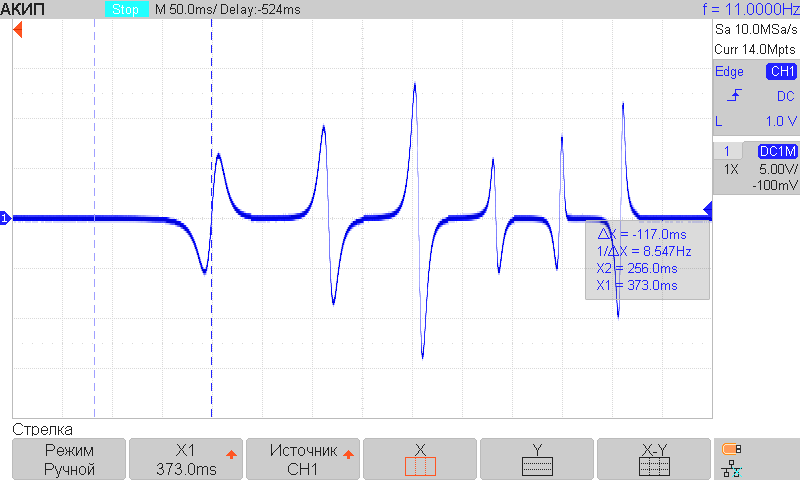
\includegraphics[scale=0.5]{AKIP0002.png}
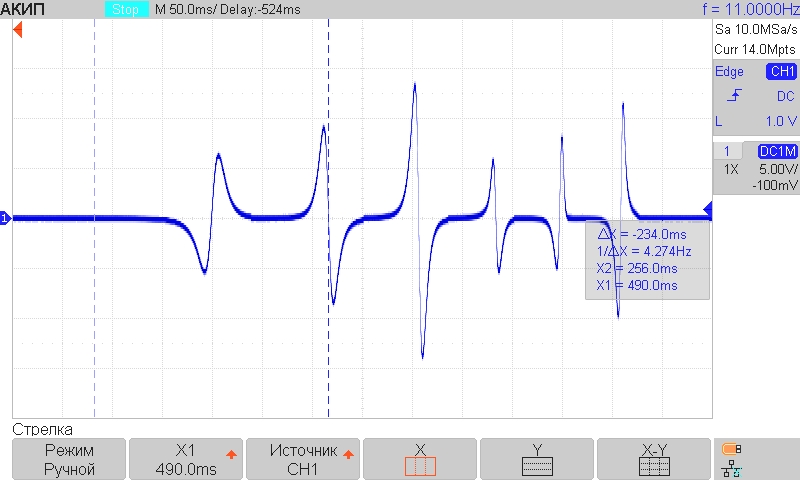
\includegraphics[scale=0.5]{AKIP0003.png}
\end{figure}

\end{document}
